\documentclass[final,hyperref={pdfpagelabels=false}]{beamer}
\usepackage{grffile}
\mode<presentation>{\usetheme{I6pd2}}
\usepackage[english]{babel}
\usepackage[latin1]{inputenc}
\usepackage{amsmath,amsthm, amssymb, latexsym}
\usepackage{multirow}
\usepackage{xcolor}
\usepackage{xspace}
\usepackage{textcomp}
%\usepackage{times}\usefonttheme{professionalfonts}  % obsolete
%\usefonttheme[onlymath]{serif}
%\boldmath
\usepackage[orientation=portrait,size=a0,scale=1.4,debug]{beamerposter}
% change list indention level
% \setdefaultleftmargin{3em}{}{}{}{}{}

\newcommand{\GeV}{\textsf{GeV}}

%\usepackage{snapshot} % will write a .dep file with all dependencies, allows for easy bundling

\usepackage{array,booktabs,tabularx}
\newcolumntype{Z}{>{\centering\arraybackslash}X} % centered tabularx columns
\newcommand{\pphantom}{\textcolor{ta3aluminium}} % phantom introduces a vertical space in p formatted table columns??!!

\setbeamercolor{headline}{fg=taaluminium,bg=black}
\setbeamertemplate{headline}{  
  \leavevmode

  \begin{beamercolorbox}[wd=\paperwidth]{headline}
    \begin{columns}[T]
      \begin{column}{.02\paperwidth}
      \end{column}
      \begin{column}{.1\paperwidth}
        \vskip4ex
        \begin{center}
          \includegraphics[width=1.1\linewidth]{}\\[6ex]
          \includegraphics[width=1.1\linewidth]{}\\[6ex]%figures/UCSanDiegoLogo-White.png}\\[6ex]
          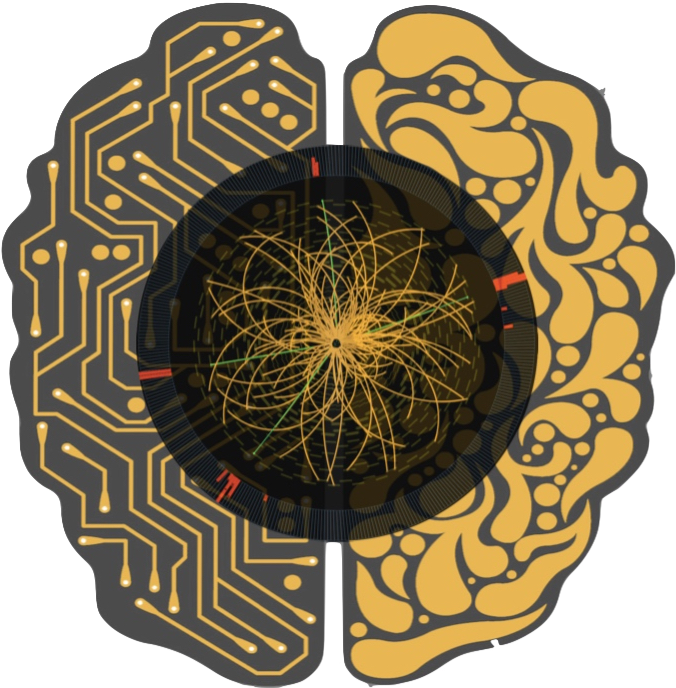
\includegraphics[width=1.1\linewidth]{figures/fml2.png}
        \end{center}
        \vskip2ex
      \end{column}
      \begin{column}{.715\paperwidth}
        \vskip8ex
        \raggedleft
        \usebeamercolor{title in headline}{\color{fg}\textbf{\huge{\inserttitle}}\\[1ex]}
        \usebeamercolor{author in headline}{\color{fg}\large{\insertauthor}\\[1ex]}
        \usebeamercolor{institute in headline}{\color{fg}\large{\insertinstitute}\\[1ex]}     
      \end{column}
      \begin{column}{.1\paperwidth}
        \vskip4ex
        \begin{center}
          \includegraphics[width=1.1\linewidth]{}\\[6ex]
          \includegraphics[width=1.1\linewidth]{}\\[6ex]
          
\includegraphics[width=\linewidth]{figures/iris-hep.png}
        \end{center}
        \vskip2ex
      \end{column}
      \begin{column}{.02\paperwidth}
      \end{column}
    \end{columns}
    \vskip2ex
  \end{beamercolorbox}

  \begin{beamercolorbox}[wd=\paperwidth]{lower separation line head}
    \rule{0pt}{3pt}
  \end{beamercolorbox}
}
%\setbeamercolor{footline}{fg=taorange, bg=black}
\setbeamerfont{footline}{size=\large,series=\tt}
\setbeamertemplate{footline}{
  \begin{beamercolorbox}[wd=\paperwidth]{upper separation line foot}
    \rule{0pt}{3pt}
  \end{beamercolorbox}
  
  \leavevmode%
  \begin{beamercolorbox}[ht=4ex,leftskip=1em,rightskip=1em]{author in
      head/foot}%
    \href{https://fastmachinelearning.org}{fastmachinelearning.org}
    \hfill
    \href{https://iris-hep.org}{iris-hep.org}
    \hfill
    \href{https://ml4physicalsciences.github.io/2020}{\textsf{Machine
        Learning and the Physical Sciences, NeurIPS 2020, Vancouver, BC, Canada}}
    \vskip1ex
  \end{beamercolorbox}
  \vskip0pt%
  \begin{beamercolorbox}[wd=\paperwidth]{lower separation line foot}
    \rule{0pt}{3pt}
  \end{beamercolorbox}
}
\setbeamercolor{separation line}{bg=taorange}
\setbeamercolor{title in headline}{fg=taaluminium}
\setbeamercolor{author in headline}{fg=taorange}
%\setbeamercolor{institute in headline}{fg=taorange}

%\setbeamercolor{framesubtitle}{fg=ta3orange, bg=ta2skyblue}
\setbeamercolor{author in head/foot}{fg=taorange, bg=black}
%\setbeamercolor{title in head/foot}{fg=taorange, bg=ta3skyblue}

\setbeamercolor*{normal text}{fg=tachameleon, bg=white}
\setbeamercolor*{block body}{fg=black,bg=white}
\setbeamercolor*{block title}{fg=taorange,bg=black}
\setbeamerfont{block title}{size=\large,series=\bf}
%\setbeamercolor{upper separation line head}{fg=ta2orange,bg=black}
%\setbeamercolor{upper separation line foot}{fg=ta2orange,bg=black}

%\setbeamercolor*{example body}{fg=ta3aluminium,bg=black}
%\setbeamercolor*{example text}{fg=ta3aluminium,bg=black}
%\setbeamercolor*{example title}{fg=ta2gray,bg=taorange}

\setbeamercolor{structure}{fg=ta3skyblue}

\listfiles

%%%%%%%%%%%%%%%%%%%%%%%%%%%%%%%%%%%%%%%%%%%%%%%%%%%%%%%%%%%%%%%%%%%%%%%%%%%%%%%%%%%%%%
\graphicspath{{figures/}}

\title{Accelerated Charged Particle Tracking with Graph Neural Networks on FPGAs}
\author{Vesal Razavimaleki{\color{lightgray}\inst{1}}, Aneesh Heintz{\color{lightgray}\inst{2}}, \href{https://jduarte.physics.ucsd.edu}{Javier Duarte}{\color{lightgray}\inst{1}}, Gage DeZoort{\color{lightgray}\inst{3}}, Isobel Ojalvo{\color{lightgray}\inst{3}}, Savannah Thais{\color{lightgray}\inst{3}}, Markus Atkinson{\color{lightgray}\inst{4}}, Mark Neubauer{\color{lightgray}\inst{4}}, Lindsey Gray{\color{lightgray}\inst{5}}, Sergo Jindariani{\color{lightgray}\inst{5}}, Nhan Tran{\color{lightgray}\inst{5}}, Phil Harris{\color{lightgray}\inst{6}}, Dylan Rankin{\color{lightgray}\inst{6}}, Thea Aarrestad{\color{lightgray}\inst{7}}, Vladimir Loncar{\color{lightgray}\inst{7}}, Maurizio Pierini{\color{lightgray}\inst{7}}, Sioni Summers{\color{lightgray}\inst{7}}, Jennifer Ngadiuba{\color{lightgray}\inst{8}}, Mia Liu{\color{lightgray}\inst{9}}, Edward Kreinar{\color{lightgray}\inst{10}}, Zhenbin Wu{\color{lightgray}\inst{11}}}
\institute{\color{lightgray}\inst{1} UC San Diego \inst{2} Cornell \inst{3} Princeton \inst{4} UIUC \inst{5} Fermilab \inst{6} MIT \inst{7} CERN \inst{8} Caltech \inst{9} Purdue \inst{10} Hawkeye360 \inst{11} UIC}
\date[December 11, 2020]{December 11, 2020}

%%%%%%%%%%%%%%%%%%%%%%%%%%%%%%%%%%%%%%%%%%%%%%%%%%%%%%%%%%%%%%%%%%%%%%%%%%%%%%%%%%%%%%
\newlength{\columnheight}
\setlength{\columnheight}{105cm}

\newcommand{\hlsfml}{{\texttt{hls4ml}}\xspace}
\newcommand{\pt}{\ensuremath{p_{\mathrm{T}}}\xspace}
\newcommand{\ptmin}{\ensuremath{p_{\mathrm{T_{min}}}}\xspace}

%%%%%%%%%%%%%%%%%%%%%%%%%%%%%%%%%%%%%%%%%%%%%%%%%%%%%%%%%%%%%%%%%%%%%%%%%%%%%%%%%%%%%%
\begin{document}
\begin{frame}
  \begin{columns}
    % ---------------------------------------------------------%
    % Set up a column 
    \begin{column}{.49\textwidth}
      \begin{beamercolorbox}[center,wd=\textwidth]{postercolumn}
        \begin{minipage}[T]{.95\textwidth}  % tweaks the width, makes a new \textwidth
          \parbox[t][\columnheight]{\textwidth}{ % must be some better way to set the the height, width and textwidth simultaneously
            % Since all columns are the same length, it is all nice and tidy.  You have to get the height empirically
            % ---------------------------------------------------------%
            % fill each column with content
            
            \begin{block}{Introduction}
                  \begin{center}
                    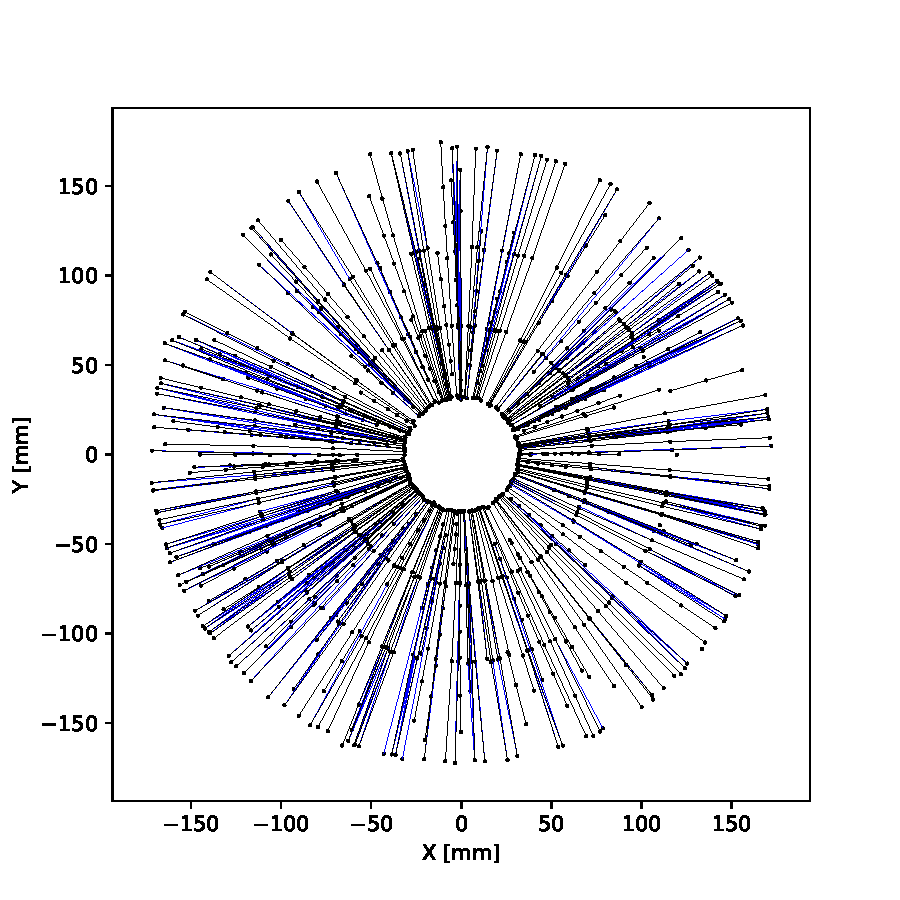
\includegraphics[width=0.33\linewidth]{figures/event000001000_section0_xy.pdf}
                     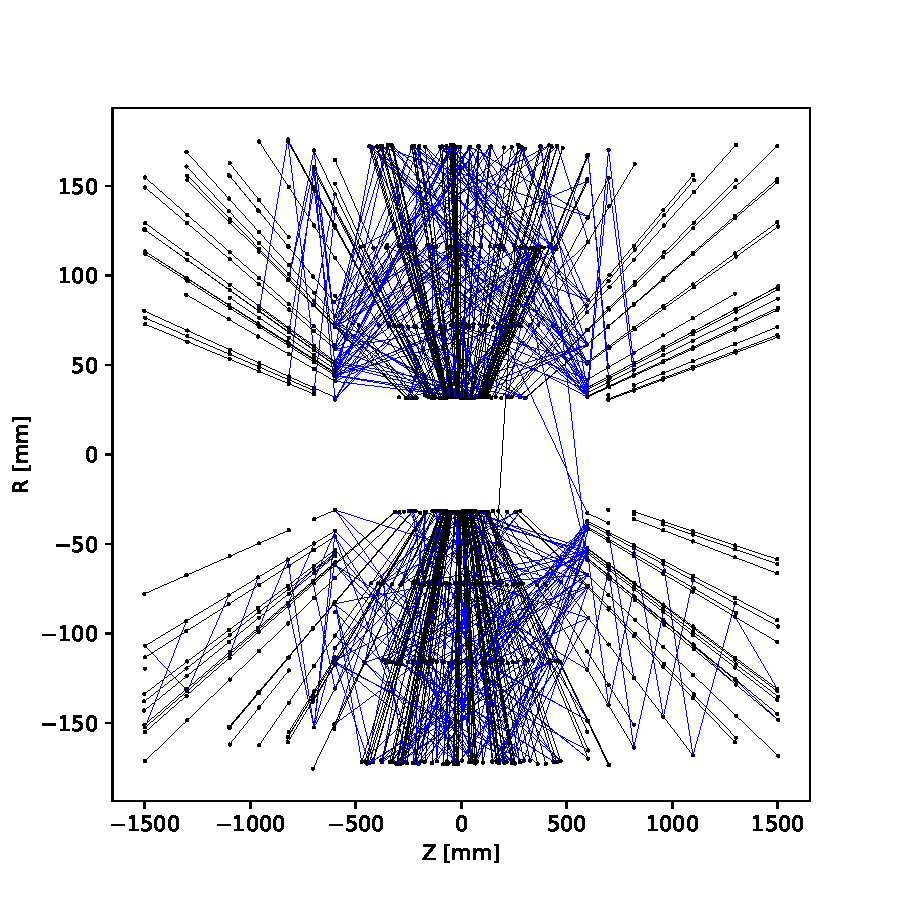
\includegraphics[width=0.33\linewidth]{figures/event000001000_section0_rz.pdf}
                  \end{center}
                  \begin{itemize}
                    \item Track reconstruction approached as a GNN "edge classification" problem
                    \item Data represented as graphs
                    \begin{itemize}
                        \item Nodes$\,\to\,$Hits
                        \item Edges$\,\to\,$Tracklet connections between hits
                    \end{itemize}
                    \item Interest in GNN inference on FPGA-based trigger systems and co-processors for offline computing
                    \item Two FPGA implementations of GNN segment classifiers explored using {\hlsfml} and OpenCL
              \end{itemize}
            \end{block}

            \begin{block}{OpenCL Implementation}
              \begin{itemize}
                \item Architecture: Interaction Network
                \begin{itemize}
                  \item Message-passing neural network (NN)
                  \item Applies separate relational and object models to update edge and node features
                \end{itemize}
              \end{itemize}
              \begin{columns}              
              \begin{column}{.49\textwidth}
                \begin{itemize}
                  \item Relational Model
                  \begin{itemize}
                    \item Fully-connected NN with 7 inputs and 4 layers (250, 250, 250, 1)
                  \end{itemize}
                  \item Object Model
                  \begin{itemize}
                    \item Fully-connected NN with 4 inputs and 3 layers (200, 200, 3)
                  \end{itemize}
                \end{itemize}
              \end{column}
            \begin{column}{.49\textwidth}
             \begin{center}
                    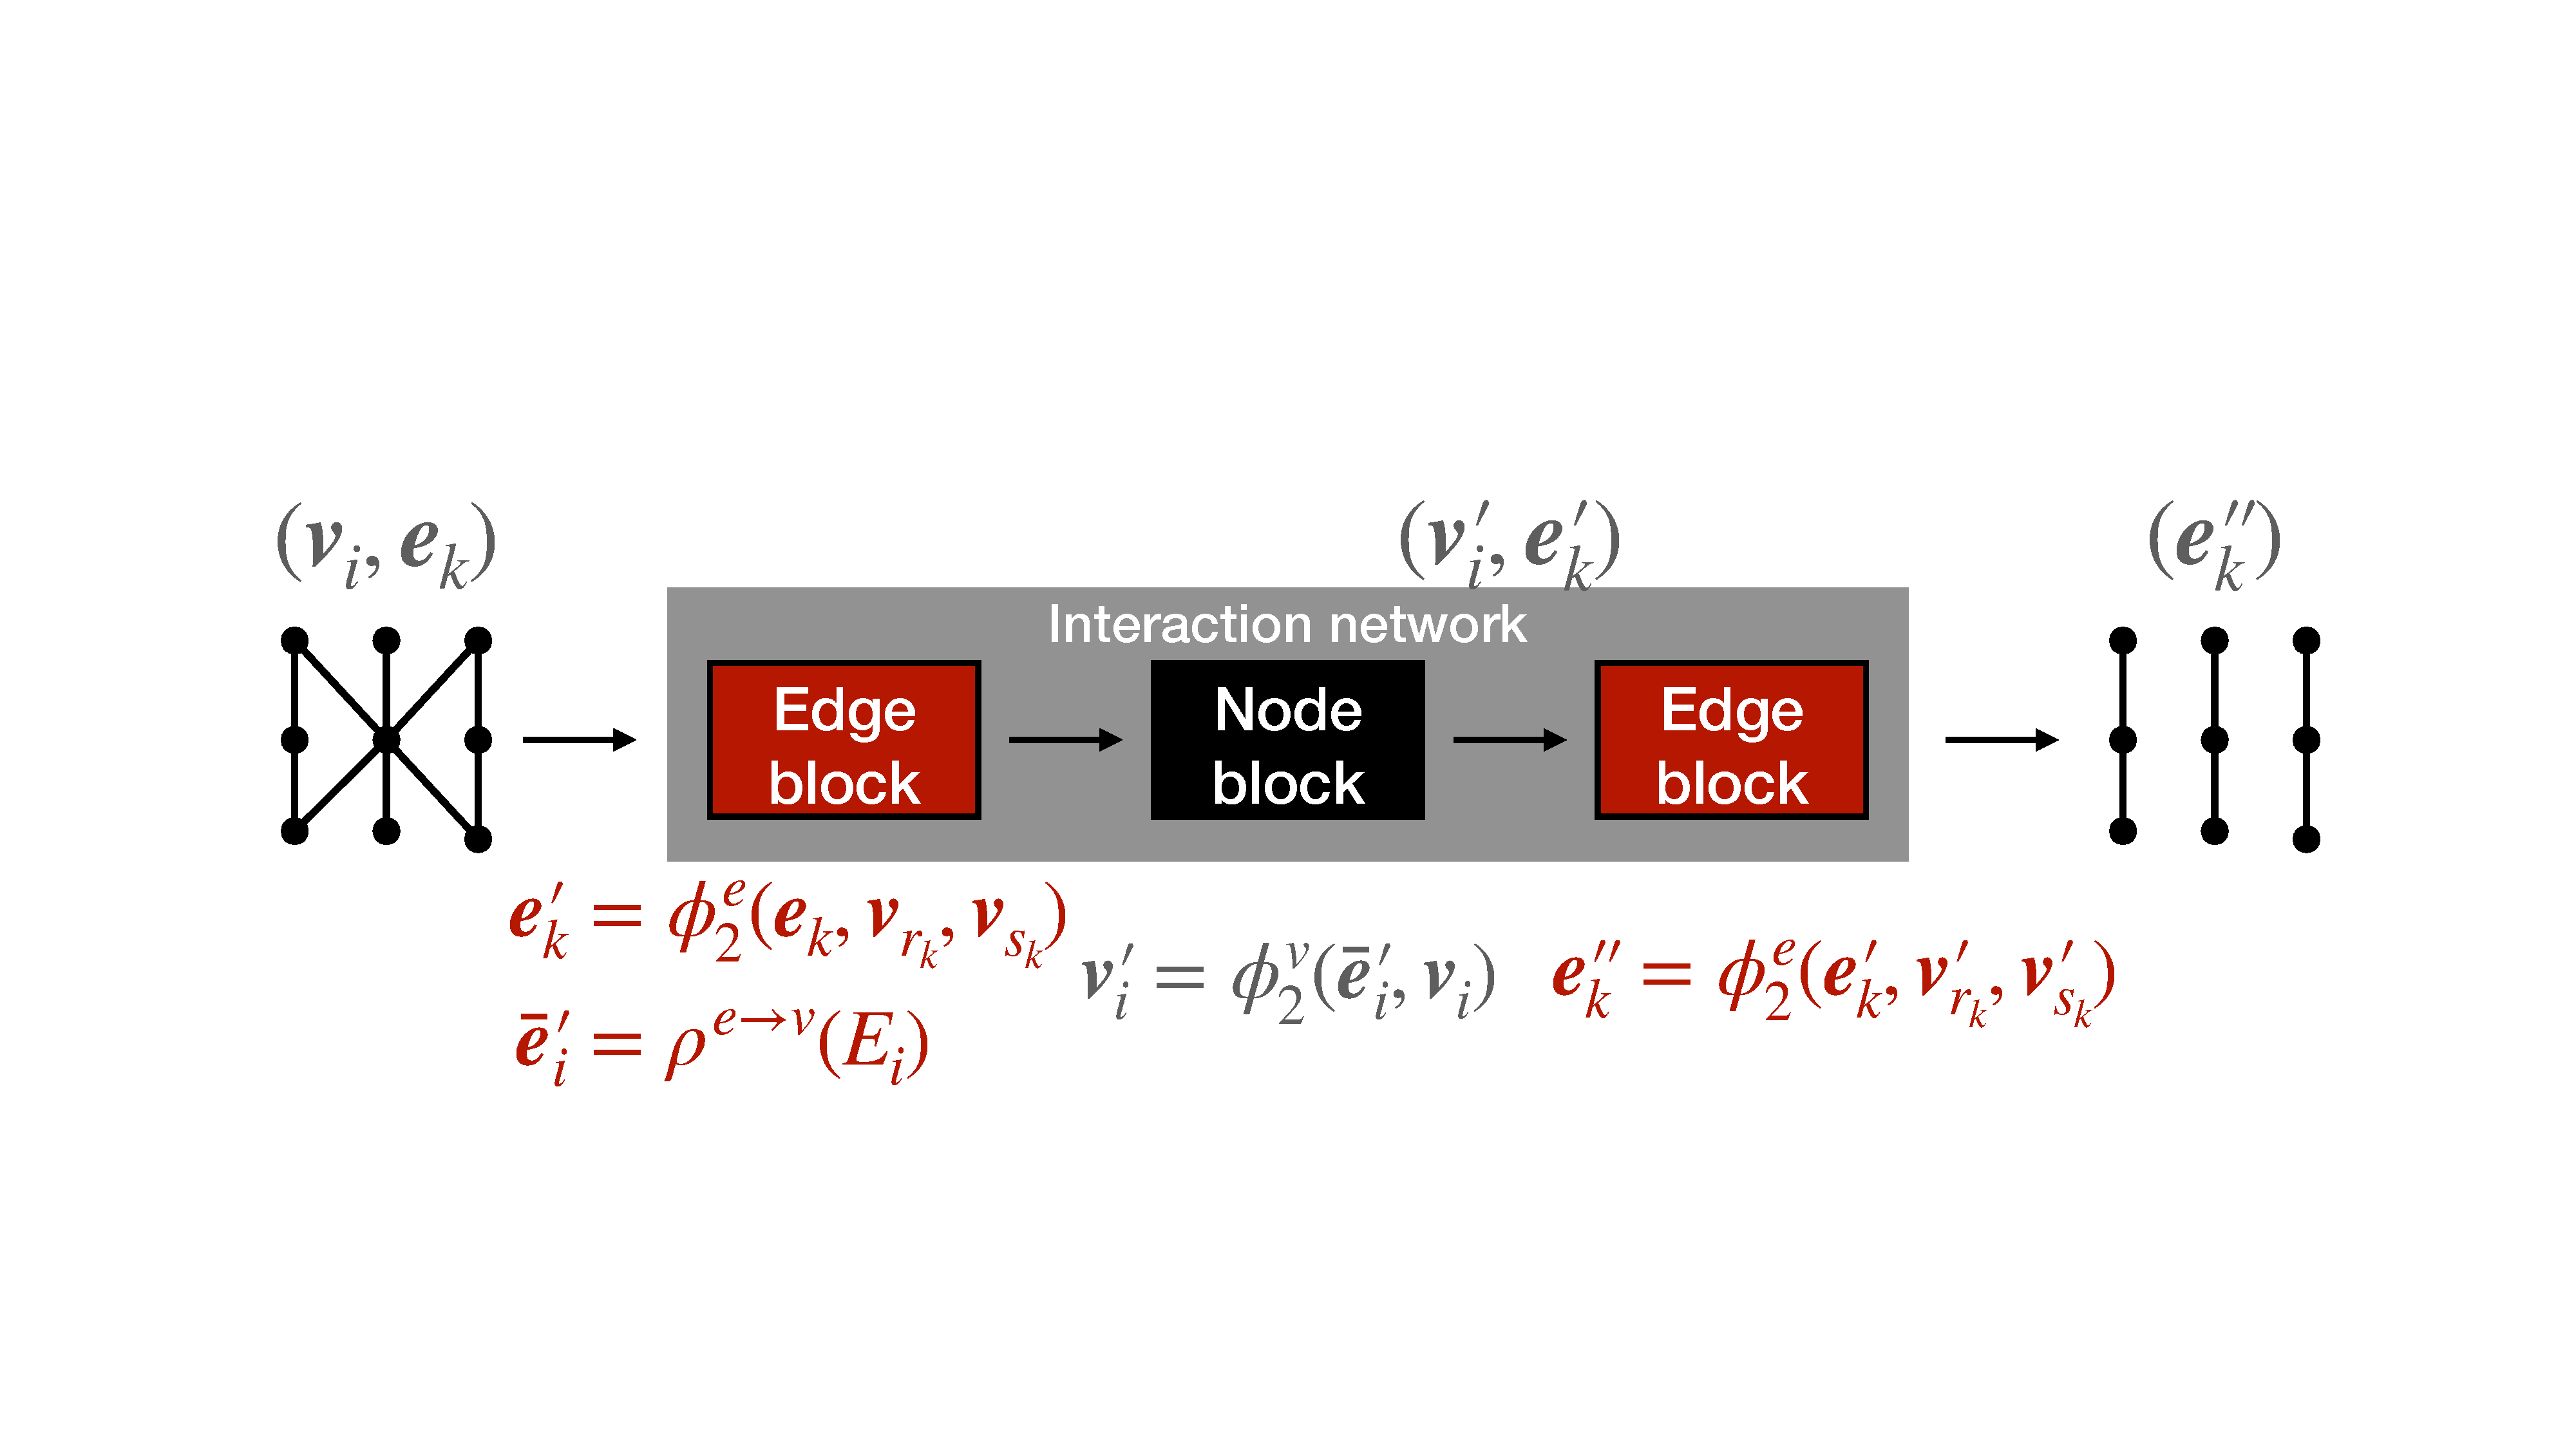
\includegraphics[width=0.9\linewidth]{OpenCL_GNN.pdf}
                  \end{center}
                \end{column}
                \end{columns}
              \end{block}
              
              \begin{block}{{\hlsfml} Implementation}
              \begin{itemize}
                \item Architecture: Exa.TrkX NeurIPS 2019 Segment Classifier
                \begin{itemize}
                  \item Encoder transforms node and edge features into an 8-dimensional latent space
                  \item Interaction network edge and node blocks update edge and node features
                  \item Decoder transforms edge features into edge classification weights
                \end{itemize}
              \end{itemize}
              \begin{columns}              
              \begin{column}{.49\textwidth}
                \begin{itemize}
                  \item Encoder
                  \begin{itemize}
                    \item Two independent, fully-connected NNs encode edges/nodes
                    \item 4/3 inputs and 2 layers (8, 8)
                  \end{itemize}
                  \item Interaction Network
                  \begin{itemize}
                    \item Edge block: 8 inputs, 2 layers (8, 8)
                    \item Node block: 8 inputs, 2 layers (8, 8)
                  \end{itemize}
                  \item Decoder
                  \begin{itemize}
                      \item Fully-connected NN with 8 inputs and 4 layers (8, 8, 8, 1)
                  \end{itemize}
                \end{itemize}
              \end{column}
              \begin{column}{.49\textwidth}
                \begin{center}
                  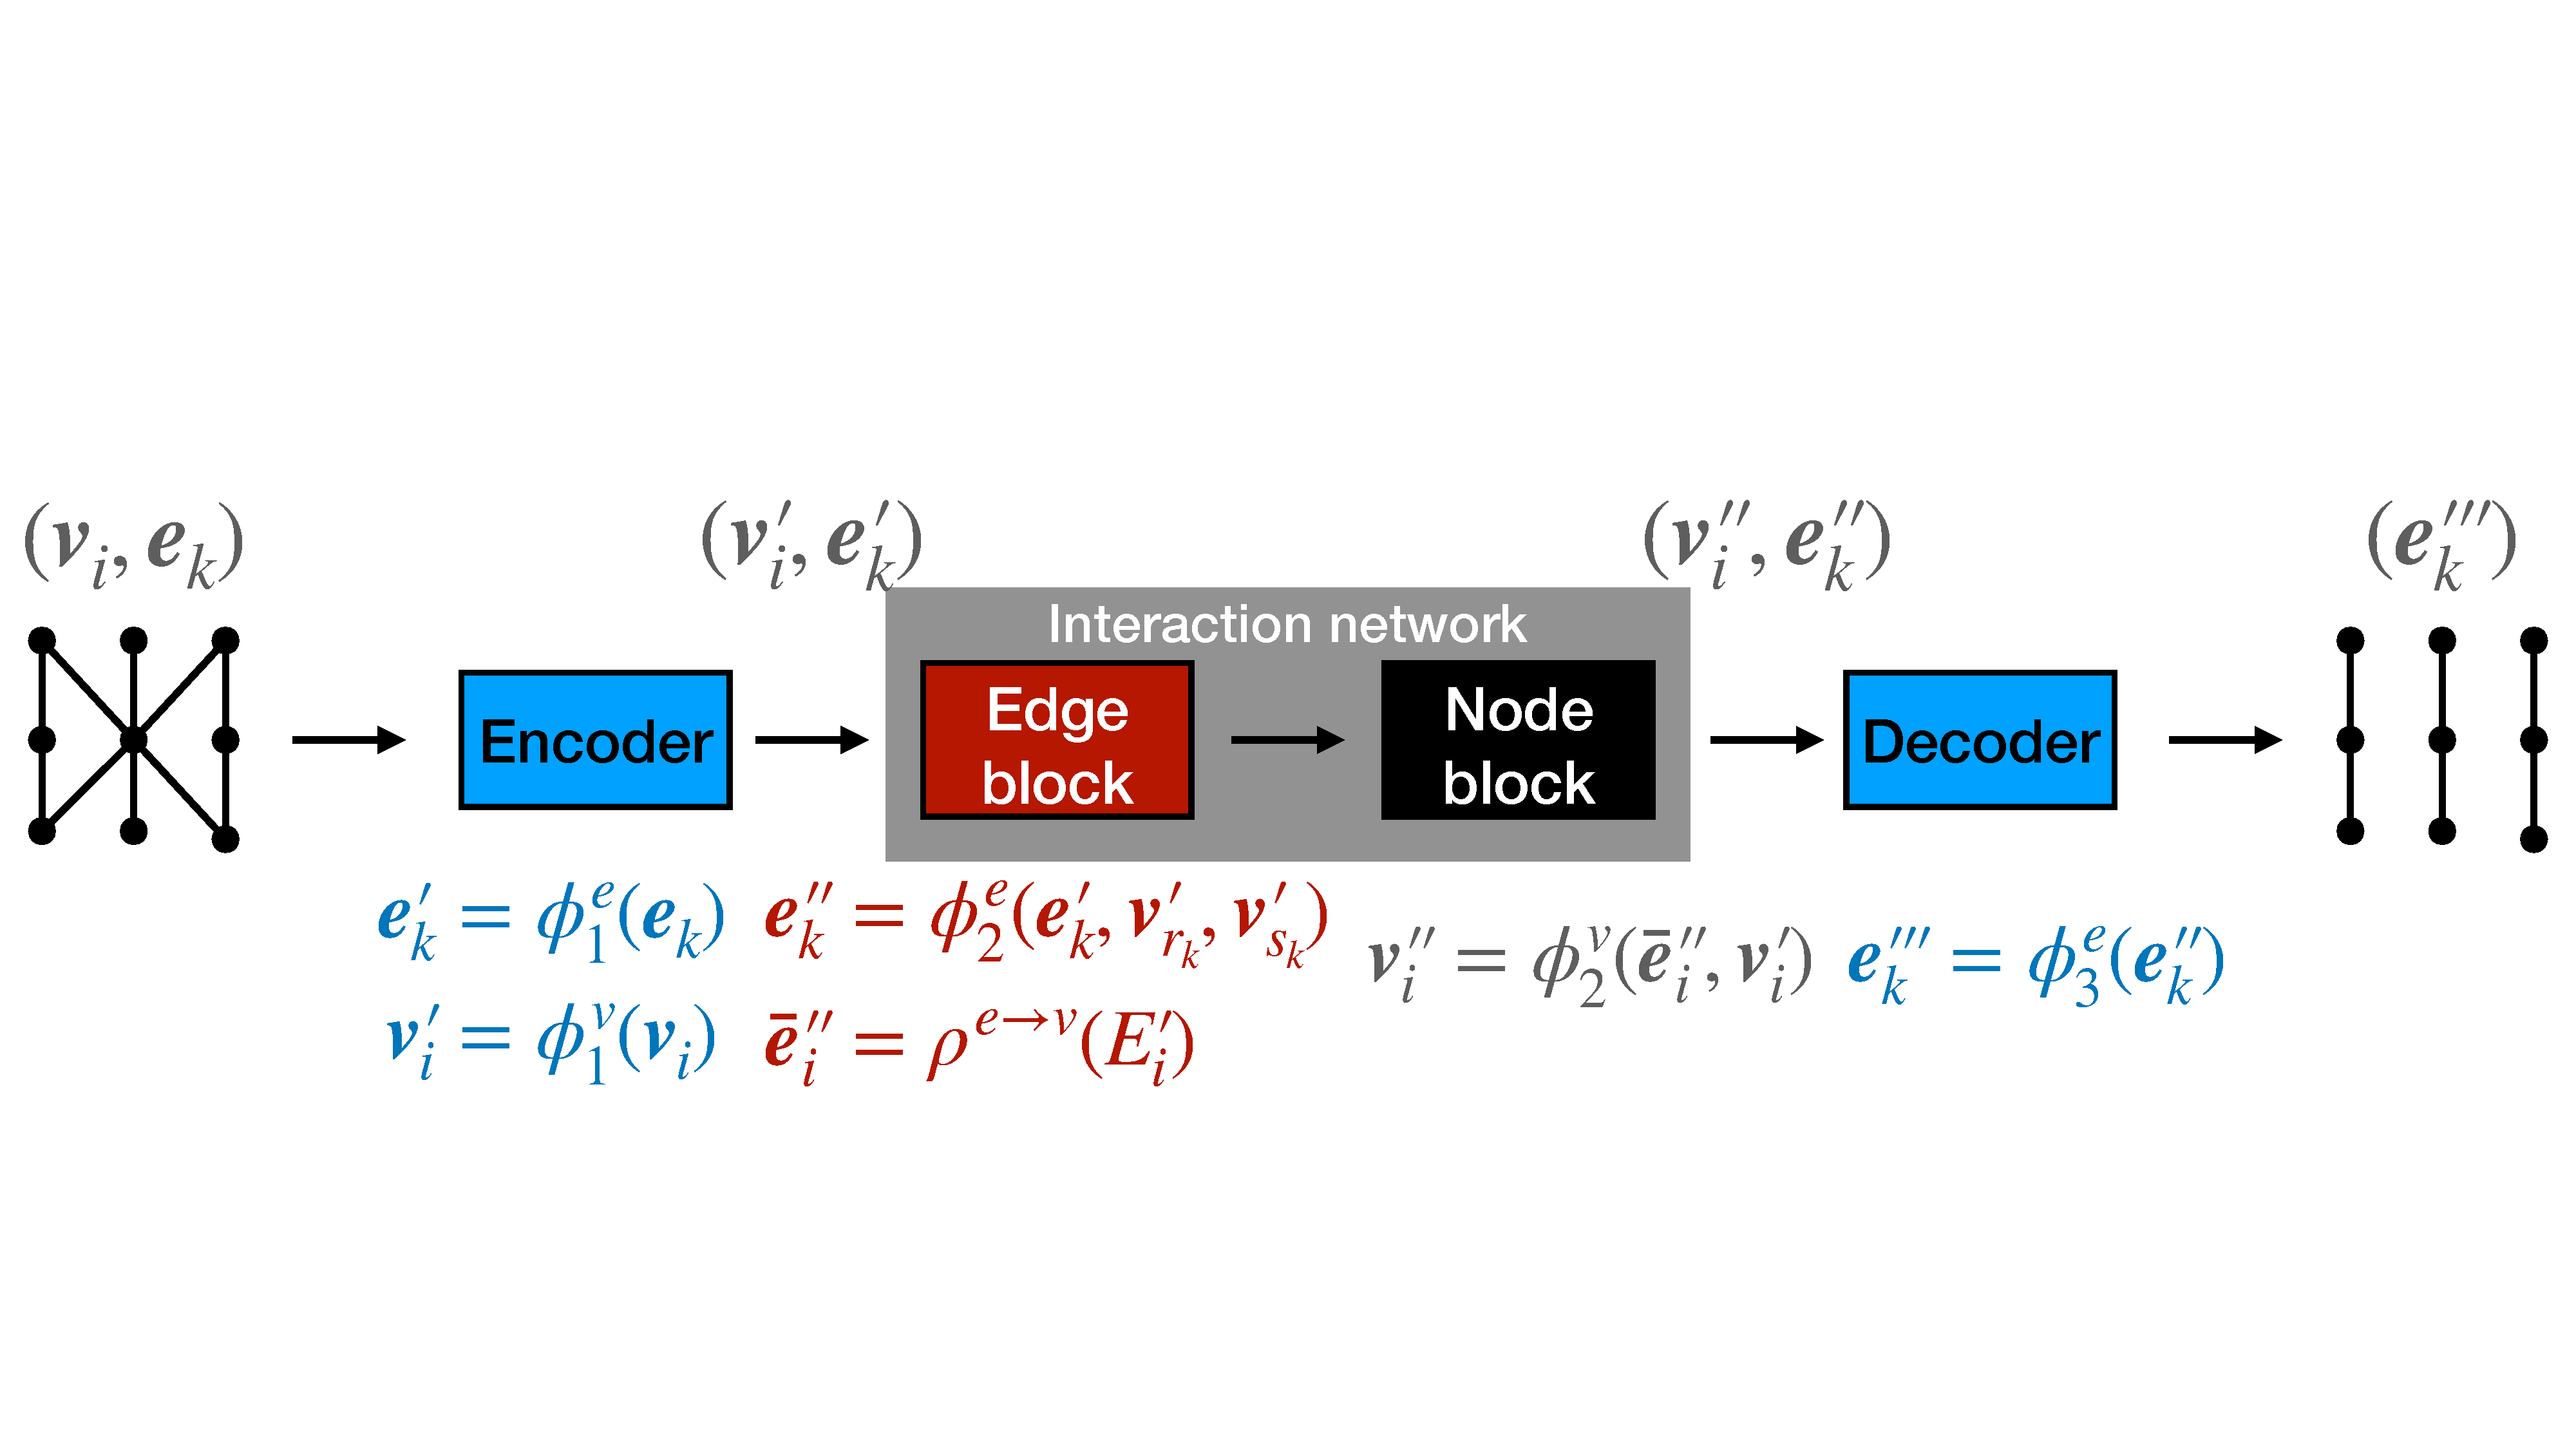
\includegraphics[width=0.9\linewidth]{hls4ml_GNN.pdf}
                \end{center}
              \end{column}
              \end{columns}
            \end{block}
            
            \begin{block}{{\hlsfml} Performance}
              \begin{itemize}
                  \item GNN can correctly classify track segments with AUC $\sim$ 0.983 \\
                  \item AUC scan vs fixed point bit precision \texttt{<total,integer>} = \texttt{<X,6>}
                  \item Good performance starting at \texttt{<12,6>}
              \end{itemize}
              \begin{columns}
                \begin{column}{.49\textwidth}
                  \begin{itemize}
                      \item Zero-padding sets max graph size
                      \item 1/16 of a TrackML detector
                      \begin{itemize}
                          \item 112 nodes, 148 edges
                          \item 95th percentile of graph sizes for \ptmin = 2~GeV
                      \end{itemize}
                  \end{itemize}
                \end{column}
                \begin{column}{.49\textwidth}
                  \begin{center}
                      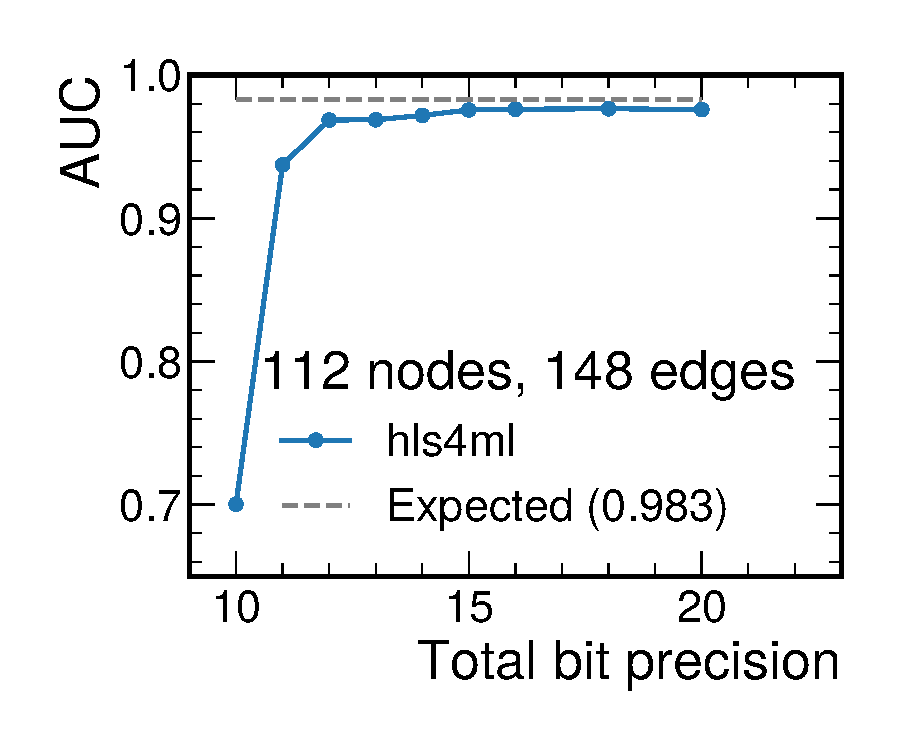
\includegraphics[width=0.673\linewidth]{figures/AUC_vs_BP.pdf}
                  \end{center}
                \end{column}
              \end{columns}
            \end{block}
              
                }
              \end{minipage}
            \end{beamercolorbox}
          \end{column}
    % ---------------------------------------------------------%
    % end the column

    % ---------------------------------------------------------%
    % Set up a column 
    \begin{column}{.49\textwidth}
      \begin{beamercolorbox}[center,wd=\textwidth]{postercolumn}
        \begin{minipage}[T]{.95\textwidth} 
          \parbox[t][\columnheight]{\textwidth}{
            
            \begin{block}{OpenCL Latency and Resources}
              \begin{itemize}
                \item Efficiency improving methods:
                \begin{itemize}
                    \item 2D local memory tiling/register blocking: reduce redundancy/latency of reading off-chip memory
                    \item Double buffering: allow host to process/transfer data while kernel executes
                    \item Loop unrolling
                \end{itemize}
                \vspace{6mm}
                \item Scales up more easily to larger graph sizes (smaller \ptmin)
                \item Achieves latency of 10~ms to 1~s
                \begin{itemize}
                    \item High due to CPU-FPGA I/O
                \end{itemize}
                \item Tested with Arria 10 GX 1150 FPGA
              \end{itemize}
              \begin{center}
                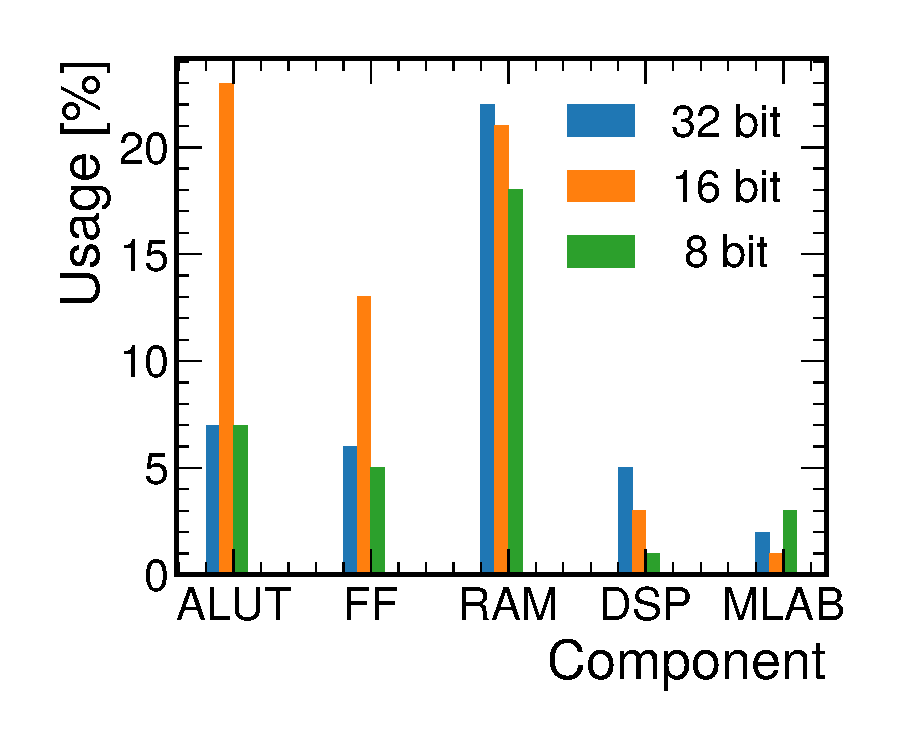
\includegraphics[width=0.33\linewidth]{resource_bit_precision_ocl.pdf}
                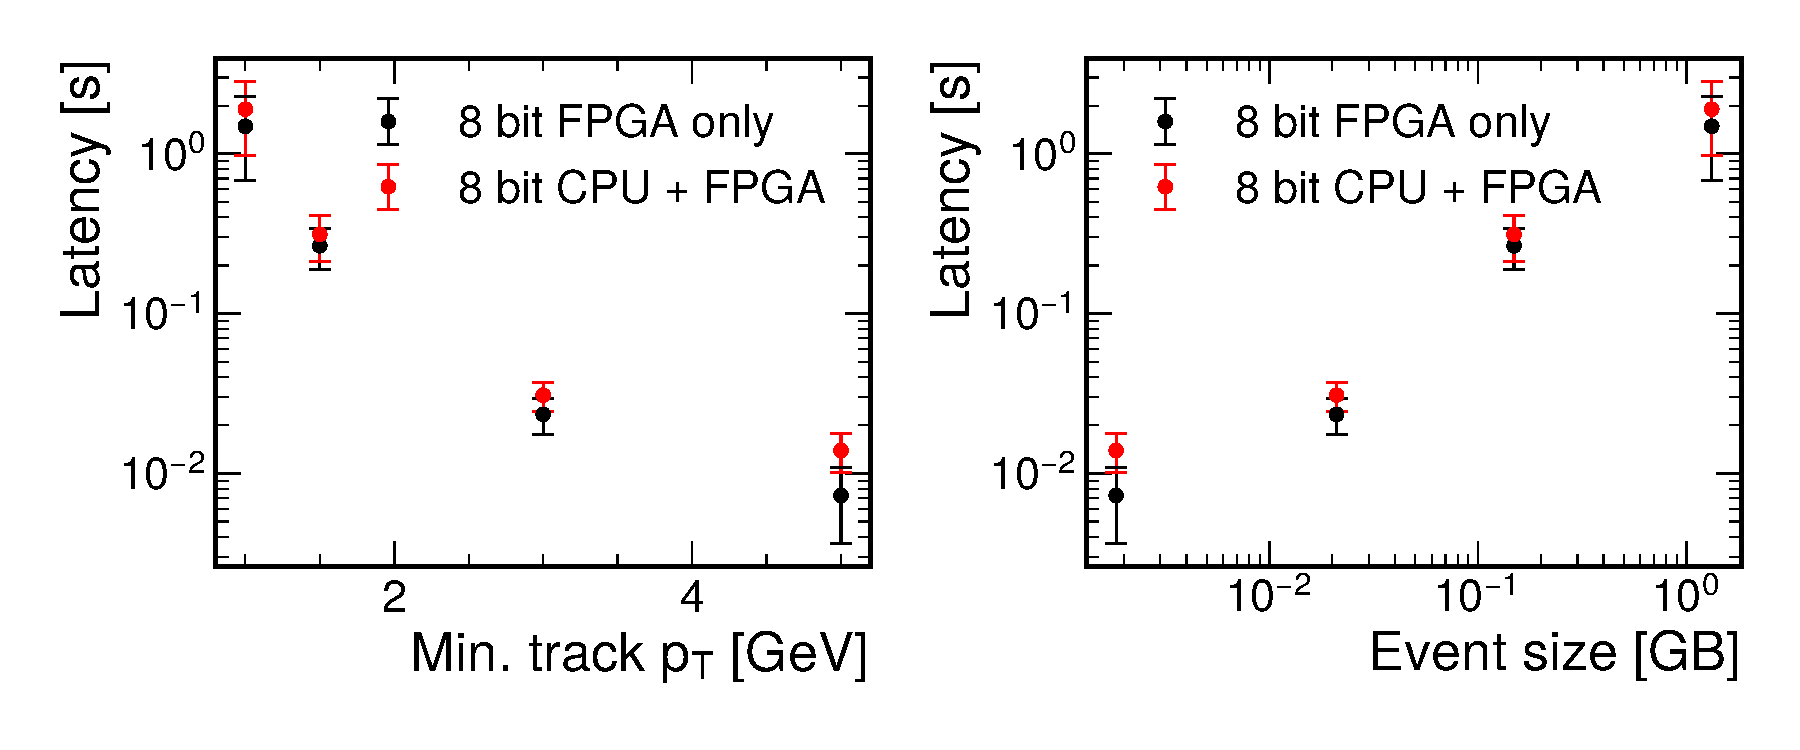
\includegraphics[width=0.66\linewidth]{scalability_study_v2.pdf}
              \end{center}
            \end{block}
            
            \begin{block}{{\hlsfml} Latency and Resources}
              \begin{itemize}
                \item Efficiency improving methods:
                \begin{itemize}
                    \item Pipelining with initiation interval = reuse factor at edge/node block-level
                    \item Input streaming: implement incoming data as FIFO to recycle resources
                    \item Loop unrolling
                \end{itemize}
                \vspace{6mm}
                \item Showing results for 1/4 of max graph size for faster scan iteration
                \begin{itemize}
                    \item 28 nodes, 37 edges with zero-padding (1/64 of TrackML detector)
                    %\item 95th percentile of graph sizes for \ptmin = 2~GeV
                \end{itemize}
                \item Achieves latency of 650~ns to 1~$\mu$s
                \item Scans vs bit precision show lower bit width results in smaller area, faster execution
                \item Scans vs reuse factor show trade-off between resource usage and latency
                \item Tested against Xilinx Kintex Ultrascale 115 FPGA
                \begin{center}
                    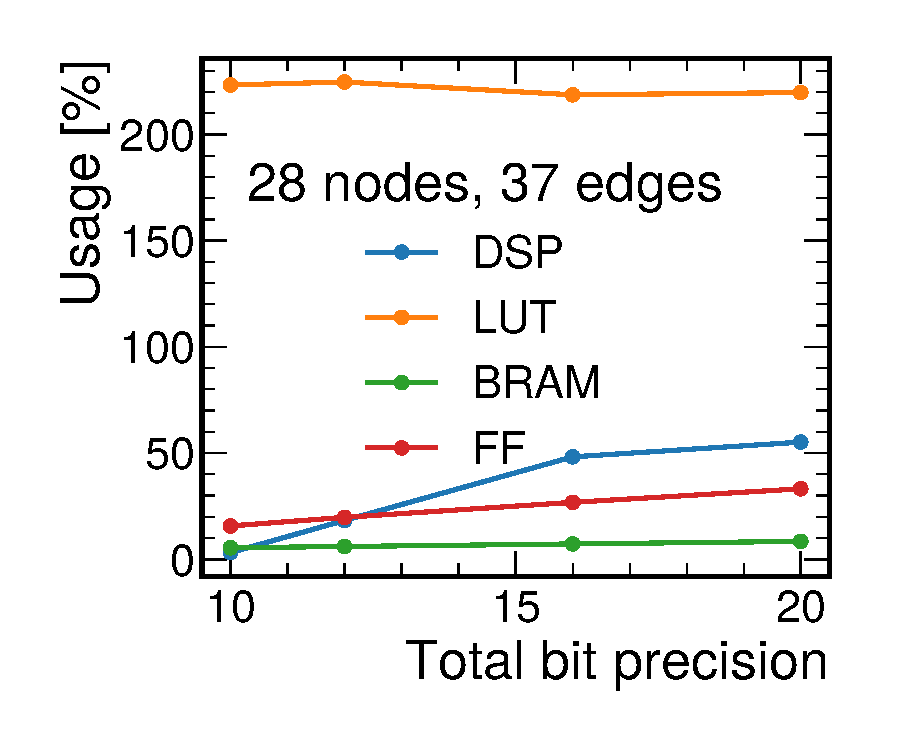
\includegraphics[width=0.33\linewidth]{Resources_vs_BP.pdf}
                    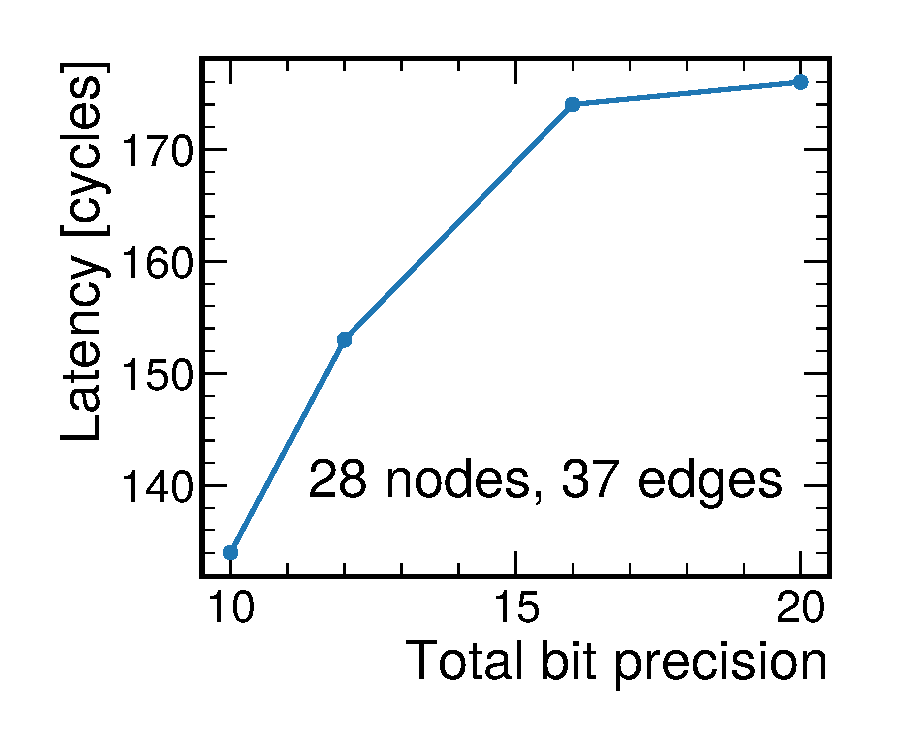
\includegraphics[width=0.33\linewidth]{Latency_vs_BP.pdf}
                    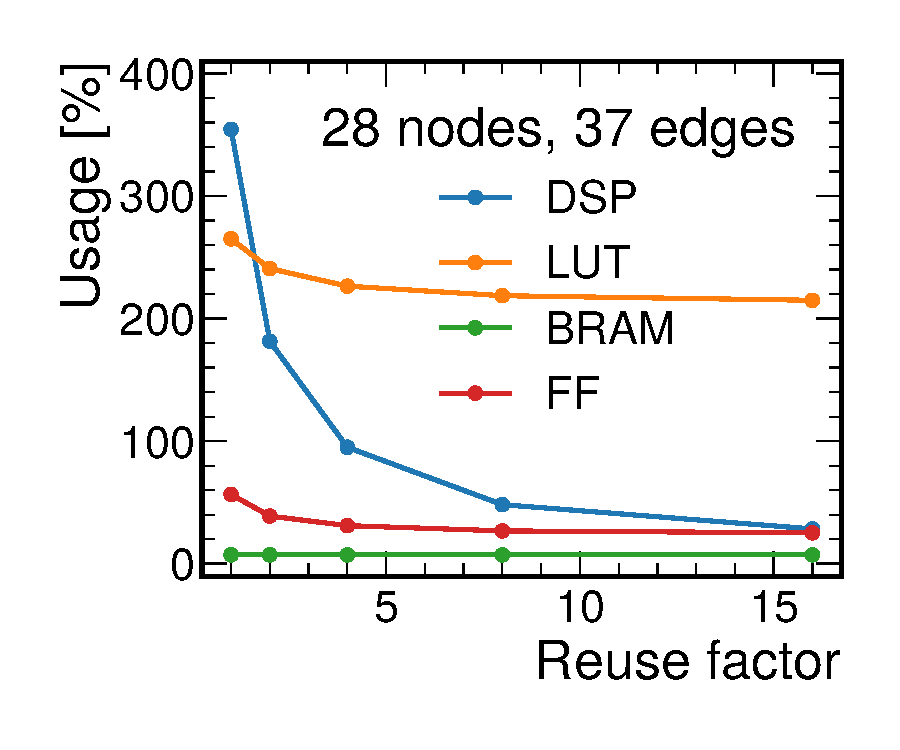
\includegraphics[width=0.33\linewidth]{Resources_vs_RF.pdf}
                    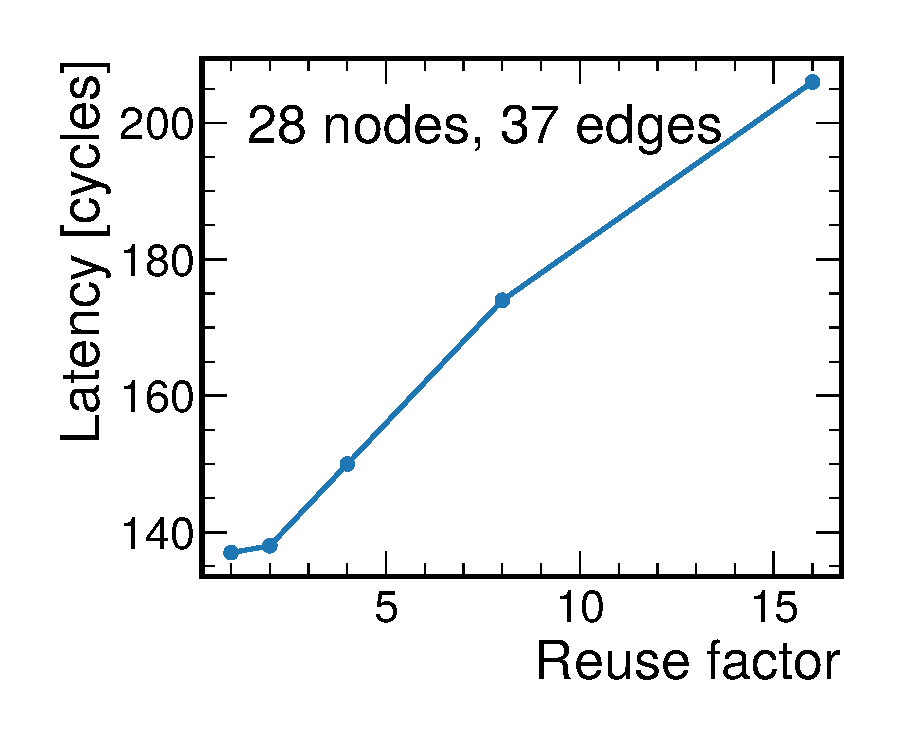
\includegraphics[width=0.33\linewidth]{Latency_vs_RF.pdf}
                \end{center}
              \end{itemize}
            \end{block}
            
            \begin{block}{Summary}
              \begin{itemize}
                \item Two complementary implementations of GNNs on FPGAs
                \item Current performance promising for trigger-level applications (\hlsfml) and co-processing applications (OpenCL and \hlsfml)
                \item OpenCL implementation scales more easily to larger graphs while {\hlsfml} implementation has latency/throughput advantage
                \item Future Work
                \begin{itemize}
                    \item Further detailed comparisons between the implementations based on the same model
                    \item Comparison with GPU co-processors
                    \item Additional optimizations such as quantization-aware training
                \end{itemize}
              \end{itemize}
                          \begin{flushright}\vspace{-3ex}
                            \href{https://arxiv.org/abs/2012.01563}{
\includegraphics[width=0.18\textwidth]{gnn_fpga_qr_code.png}}
                          \end{flushright}
                  \end{block}                  
          }
          % ---------------------------------------------------------%
          % end the column
        \end{minipage}
      \end{beamercolorbox}
    \end{column}
    % ---------------------------------------------------------%
    % end the column
  \end{columns}
  \vskip1ex

\end{frame}
\end{document}


%%%%%%%%%%%%%%%%%%%%%%%%%%%%%%%%%%%%%%%%%%%%%%%%%%%%%%%%%%%%%%%%%%%%%%%%%%%%%%%%%%%%%%%%%%%%%%%%%%%%
%%% Local Variables: 
%%% mode: latex
%%% TeX-PDF-mode: t
%%% End: